\documentclass[12pt,a4paper]{article}

% Packages
\usepackage[utf8]{inputenc}
\usepackage[T1]{fontenc}
\usepackage{geometry}
\usepackage{graphicx}
\usepackage{float}
\usepackage{amsmath}
\usepackage{amssymb}
\usepackage{hyperref}
\usepackage{listings}
\usepackage{xcolor}
\usepackage{enumitem}
\usepackage{titlesec}
\usepackage{fancyhdr}
\usepackage{tcolorbox}
\usepackage{booktabs}
\usepackage{tikz}
\usepackage{caption}
\usepackage{subcaption}

% Page geometry
\geometry{
    a4paper,
    top=2.5cm,
    bottom=2.5cm,
    left=2.5cm,
    right=2.5cm
}

% Header and footer
\pagestyle{fancy}
\fancyhf{}
\fancyhead[L]{AIN4312 - Checkpoint 2}
\fancyhead[R]{AI Energy Optimization}
\fancyfoot[C]{\thepage}
\renewcommand{\headrulewidth}{0.5pt}
\renewcommand{\footrulewidth}{0.5pt}

% Colors
\definecolor{codebackground}{RGB}{248, 248, 248}
\definecolor{codekeyword}{RGB}{0, 102, 204}
\definecolor{codestring}{RGB}{204, 102, 0}
\definecolor{codecomment}{RGB}{102, 102, 102}
\definecolor{primarycolor}{RGB}{255, 107, 53}
\definecolor{secondarycolor}{RGB}{46, 196, 182}

% Code listing style
\lstdefinestyle{mystyle}{
    backgroundcolor=\color{codebackground},
    commentstyle=\color{codecomment}\itshape,
    keywordstyle=\color{codekeyword}\bfseries,
    stringstyle=\color{codestring},
    basicstyle=\ttfamily\footnotesize,
    breakatwhitespace=false,
    breaklines=true,
    captionpos=b,
    keepspaces=true,
    numbers=left,
    numbersep=5pt,
    showspaces=false,
    showstringspaces=false,
    showtabs=false,
    tabsize=4,
    frame=single,
    rulecolor=\color{black!30}
}
\lstset{style=mystyle}

% Title formatting
\titleformat{\section}
  {\normalfont\Large\bfseries\color{primarycolor}}
  {\thesection}{1em}{}

\titleformat{\subsection}
  {\normalfont\large\bfseries\color{secondarycolor}}
  {\thesubsection}{1em}{}

% Hyperref setup
\hypersetup{
    colorlinks=true,
    linkcolor=primarycolor,
    urlcolor=secondarycolor,
    citecolor=primarycolor,
    pdftitle={Checkpoint 2 - Frontend and API Integration},
    pdfauthor={AI Energy Optimization Team}
}

% Document information
\title{
    \vspace{-1cm}
    \huge\textbf{AIN4312 - Checkpoint 2}\\
    \vspace{0.5cm}
    \Large\textbf{Frontend Development \& API Integration}\\
    \vspace{0.3cm}
    \large AI Energy Optimization for Smart Homes\\
    \vspace{0.2cm}
}
\author{
    AI Energy Optimization Team\\
    \small \href{https://github.com/WajeehAlamoudi/AI\_energy\_optimization}{GitHub Repository}
}
\date{\today}

\begin{document}

\maketitle
\thispagestyle{fancy}

% Abstract/Executive Summary
\begin{tcolorbox}[colback=primarycolor!5, colframe=primarycolor, title=Executive Summary]
This document presents Checkpoint 2 of the AI Energy Optimization project, focusing on the \textbf{frontend development} and \textbf{API integration}. The checkpoint demonstrates the complete implementation of a web-based dashboard connected to a FastAPI backend, enabling users to monitor and control AI-driven energy optimization in smart homes. The system architecture combines modern web technologies with RESTful API design to create an intuitive, responsive, and powerful interface for managing homes, devices, and reinforcement learning training processes.
\end{tcolorbox}

\vspace{0.5cm}

\tableofcontents
\newpage

%=============================================================================
\section{Introduction}
%=============================================================================

This checkpoint represents a critical milestone in the AI Energy Optimization project, where we transition from backend algorithms and machine learning models to a \textbf{user-facing application}. The primary objective is to create a seamless connection between the sophisticated AI/ML backend and an intuitive web interface.

\subsection{Project Context}

The AI Energy Optimization system is designed to:
\begin{itemize}[leftmargin=*]
    \item Simulate smart home environments with multiple rooms and devices
    \item Use reinforcement learning (DQN) to learn optimal energy-saving policies
    \item Predict temperature and energy consumption using XGBoost models
    \item Provide real-time monitoring and control through a web dashboard
\end{itemize}

\subsection{Checkpoint 2 Objectives}

This checkpoint specifically focuses on:
\begin{enumerate}[leftmargin=*]
    \item \textbf{Frontend Architecture}: Design and implementation of a modern, responsive web interface
    \item \textbf{API Development}: Creation of RESTful endpoints for all system operations
    \item \textbf{Integration Layer}: Seamless communication between frontend and backend
    \item \textbf{User Experience}: Intuitive controls for home management, device configuration, and AI training
\end{enumerate}

%=============================================================================
\section{Technology Stack}
%=============================================================================

\subsection{Backend Technologies}

\begin{table}[H]
\centering
\begin{tabular}{@{}ll@{}}
\toprule
\textbf{Technology} & \textbf{Purpose} \\ \midrule
FastAPI & RESTful API framework \\
Uvicorn & ASGI web server \\
Python 3.10+ & Primary programming language \\
PyTorch & Deep learning (DQN agent) \\
XGBoost & Gradient boosting (predictions) \\
Pandas & Data manipulation \\
NumPy & Numerical computations \\ \bottomrule
\end{tabular}
\caption{Backend technology stack}
\label{tab:backend-stack}
\end{table}

\subsection{Frontend Technologies}

\begin{table}[H]
\centering
\begin{tabular}{@{}ll@{}}
\toprule
\textbf{Technology} & \textbf{Purpose} \\ \midrule
HTML5 & Document structure \\
CSS3 & Styling and animations \\
Vanilla JavaScript & Client-side logic \\
Fetch API & HTTP requests \\
SVG & Vector graphics \\ \bottomrule
\end{tabular}
\caption{Frontend technology stack}
\label{tab:frontend-stack}
\end{table}

\subsection{Design Philosophy}

The frontend is built using \textbf{Vanilla JavaScript} without frameworks like React or Vue.js. This decision was made to:
\begin{itemize}[leftmargin=*]
    \item Minimize dependencies and reduce bundle size
    \item Demonstrate core web development principles
    \item Ensure fast loading times
    \item Maintain simplicity for educational purposes
\end{itemize}

The design follows the \textbf{"Aura Energy"} theme with:
\begin{itemize}[leftmargin=*]
    \item Warm earth tones (Orange \#FF6B35, Teal \#2EC4B6, Beige \#F7C59F)
    \item Glassmorphism effects for modern aesthetics
    \item Smooth animations and transitions
    \item Responsive layout for all screen sizes
\end{itemize}

%=============================================================================
\section{System Architecture}
%=============================================================================

\subsection{High-Level Architecture}

The system follows a classic \textbf{client-server architecture} with clear separation of concerns:

\begin{figure}[H]
\centering
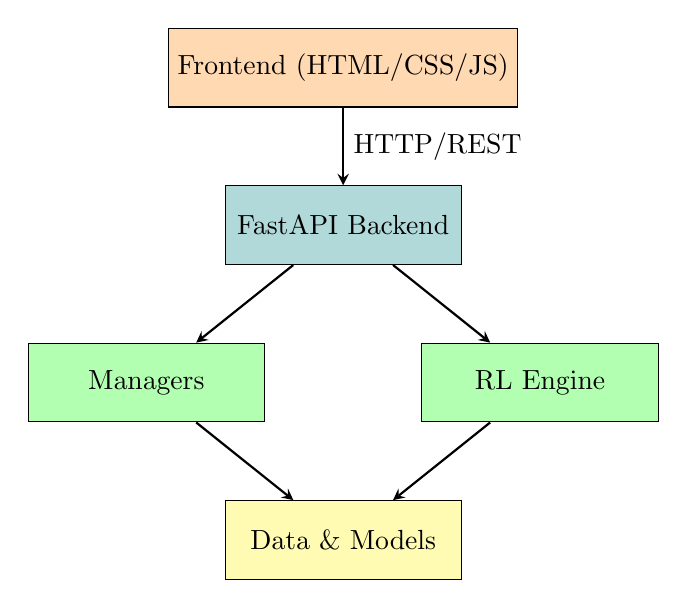
\begin{tikzpicture}[
    box/.style={rectangle, draw, fill=blue!20, minimum width=3cm, minimum height=1cm},
    arrow/.style={->, >=stealth, thick}
]
    % Frontend layer
    \node[box, fill=orange!30] (frontend) at (0, 4) {Frontend (HTML/CSS/JS)};
    
    % API layer
    \node[box, fill=teal!30] (api) at (0, 2) {FastAPI Backend};
    
    % Business logic layer
    \node[box, fill=green!30] (managers) at (-2.5, 0) {Managers};
    \node[box, fill=green!30] (rl) at (2.5, 0) {RL Engine};
    
    % Data layer
    \node[box, fill=yellow!30] (data) at (0, -2) {Data \& Models};
    
    % Arrows
    \draw[arrow] (frontend) -- node[right] {HTTP/REST} (api);
    \draw[arrow] (api) -- (managers);
    \draw[arrow] (api) -- (rl);
    \draw[arrow] (managers) -- (data);
    \draw[arrow] (rl) -- (data);
\end{tikzpicture}
\caption{System architecture diagram}
\label{fig:architecture}
\end{figure}

\subsection{Component Breakdown}

\subsubsection{Frontend Layer}
\begin{itemize}[leftmargin=*]
    \item \texttt{index.html}: Single-page application structure with multiple views
    \item \texttt{styles.css}: Complete styling with animations and responsive design
    \item \texttt{script.js}: Main application logic and event handling
    \item \texttt{data.js}: API integration and data fetching utilities
\end{itemize}

\subsubsection{API Layer}
\begin{itemize}[leftmargin=*]
    \item \texttt{app.py}: FastAPI application with all endpoint definitions
    \item RESTful design following HTTP standards
    \item CORS middleware for cross-origin requests
    \item Static file serving for frontend assets
\end{itemize}

\subsubsection{Business Logic Layer}
\begin{itemize}[leftmargin=*]
    \item \texttt{HomeManager}: Home and room configuration
    \item \texttt{DeviceManager}: Device catalog management
    \item \texttt{ImpactCalibrator}: Energy/temperature impact calculations
    \item \texttt{RLAgent}: DQN reinforcement learning agent
    \item \texttt{SmartHomeEnv}: Simulation environment
\end{itemize}

%=============================================================================
\section{Frontend Implementation}
%=============================================================================

\subsection{User Interface Structure}

The application consists of a \textbf{single-page application (SPA)} with multiple views:

\begin{enumerate}[leftmargin=*]
    \item \textbf{Welcome Screen}: Initial loading and system initialization
    \item \textbf{Overview}: Dashboard with energy metrics and quick actions
    \item \textbf{Homes}: Home and room management interface
    \item \textbf{Devices}: Device catalog and configuration
    \item \textbf{Training}: AI training control panel
    \item \textbf{Analytics}: Performance metrics and visualizations
\end{enumerate}

\subsection{Welcome Screen}

The welcome screen serves as the entry point with animated logo and system initialization:

\begin{lstlisting}[language=HTML, caption=Welcome screen structure]
<div id="welcome-screen" class="screen active">
    <div class="welcome-content">
        <div class="logo-container">
            <svg class="logo-icon" viewBox="0 0 100 100">
                <!-- Animated concentric circles -->
            </svg>
        </div>
        <h1 class="welcome-title">Aura Energy</h1>
        <p class="welcome-subtitle">Intelligent Home Optimization</p>
        <div class="welcome-stats">
            <div class="stat-pill">
                <span id="init-homes">--</span>
                <span>Homes</span>
            </div>
            <div class="stat-pill">
                <span id="init-devices">--</span>
                <span>Devices</span>
            </div>
        </div>
        <button class="enter-btn" id="enter-app">
            Enter Dashboard
        </button>
    </div>
</div>
\end{lstlisting}

\subsection{Navigation System}

The top navigation bar provides:
\begin{itemize}[leftmargin=*]
    \item Branding with animated logo
    \item Tab-based view switching
    \item Real-time weather information
    \item Responsive design for mobile devices
\end{itemize}

\begin{lstlisting}[language=JavaScript, caption=View switching logic]
// Tab navigation implementation
document.querySelectorAll('.nav-tab').forEach(tab => {
    tab.addEventListener('click', () => {
        const viewName = tab.dataset.view;
        
        // Update active tab
        document.querySelectorAll('.nav-tab').forEach(t => 
            t.classList.remove('active'));
        tab.classList.add('active');
        
        // Switch view
        document.querySelectorAll('.view').forEach(v => 
            v.classList.remove('active'));
        document.getElementById(`view-${viewName}`)
            .classList.add('active');
    });
});
\end{lstlisting}

\subsection{Styling and Design}

\subsubsection{Color Palette}
The design uses a carefully selected color palette:
\begin{itemize}[leftmargin=*]
    \item \textbf{Primary Orange}: \#FF6B35 - Energy and warmth
    \item \textbf{Secondary Teal}: \#2EC4B6 - Technology and efficiency
    \item \textbf{Beige}: \#F7C59F - Comfort and balance
    \item \textbf{Light Background}: \#EFEFD0 - Clean and modern
\end{itemize}

\subsubsection{Glassmorphism Effect}
Modern glass-like cards with backdrop blur:

\begin{lstlisting}[language=CSS, caption=Glassmorphism card styling]
.card {
    background: rgba(255, 255, 255, 0.7);
    backdrop-filter: blur(20px);
    border: 1px solid rgba(255, 255, 255, 0.3);
    border-radius: 16px;
    padding: 1.5rem;
    box-shadow: 0 8px 32px rgba(0, 0, 0, 0.1);
    transition: all 0.3s cubic-bezier(0.4, 0, 0.2, 1);
}

.card:hover {
    transform: translateY(-4px);
    box-shadow: 0 12px 48px rgba(0, 0, 0, 0.15);
}
\end{lstlisting}

\subsubsection{Animated Background}
Dynamic gradient orbs create an engaging atmosphere:

\begin{lstlisting}[language=CSS, caption=Animated gradient orbs]
.gradient-orb {
    position: absolute;
    border-radius: 50%;
    filter: blur(80px);
    opacity: 0.6;
    animation: float 20s ease-in-out infinite;
}

.orb-1 {
    background: radial-gradient(circle, #FF6B35, transparent);
    width: 500px;
    height: 500px;
    top: -10%;
    left: -5%;
}

@keyframes float {
    0%, 100% { transform: translate(0, 0) scale(1); }
    33% { transform: translate(30px, -30px) scale(1.1); }
    66% { transform: translate(-20px, 20px) scale(0.9); }
}
\end{lstlisting}

%=============================================================================
\section{API Development}
%=============================================================================

\subsection{RESTful API Design}

The API follows REST principles with clear resource-based endpoints and appropriate HTTP methods:

\begin{table}[H]
\centering
\small
\begin{tabular}{@{}p{2.5cm}p{4cm}p{5.5cm}@{}}
\toprule
\textbf{Method} & \textbf{Endpoint} & \textbf{Description} \\ \midrule
GET & /api/init & Initialize system (calibration) \\
GET & /api/homes & List all homes \\
POST & /api/homes/add & Create a new home \\
POST & /api/homes/delete & Remove a home \\
POST & /api/rooms/add & Add room to home \\
POST & /api/rooms/delete & Remove room from home \\
POST & /api/rooms/assign\_device & Assign device to room \\
GET & /api/devices & List all devices \\
POST & /api/devices/add & Add new device \\
GET & /api/weather & Get current weather \\
POST & /api/train & Train RL agent \\
POST & /api/simulate/day & Run 24h simulation \\
GET & /api/kpis & Get KPI summary \\
GET & /api/kpis/full & Get complete KPI log \\ \bottomrule
\end{tabular}
\caption{Complete API endpoint list}
\label{tab:api-endpoints}
\end{table}

\subsection{Endpoint Implementation}

\subsubsection{System Initialization}

\begin{lstlisting}[language=Python, caption=System initialization endpoint]
@app.get("/api/init")
def init_system():
    """
    Initializes the system by:
    1. Running impact calibration
    2. Loading device and home managers
    3. Returning system statistics
    """
    calibrator = ImpactCalibrator()
    calibrator.calibrate()
    devices = DeviceManager()
    homes = HomeManager()
    
    return {
        "message": "System initialized successfully",
        "devices_count": len(devices.get_all_devices()),
        "homes_count": len(homes.homes)
    }
\end{lstlisting}

\subsubsection{Home Management}

\begin{lstlisting}[language=Python, caption=Home management endpoints]
@app.get("/api/homes")
def list_homes():
    """Returns all configured homes with rooms and devices"""
    manager = HomeManager()
    return manager.homes

@app.post("/api/homes/add")
def add_home(
    home_name: str = Body(...), 
    comfort_range: tuple = Body((21, 25))
):
    """
    Creates a new home with specified comfort range
    
    Args:
        home_name: Name of the home
        comfort_range: (min_temp, max_temp) tuple
    """
    manager = HomeManager()
    return manager.add_home(home_name, comfort_range)
\end{lstlisting}

\subsubsection{Device Management}

\begin{lstlisting}[language=Python, caption=Device catalog endpoint]
@app.get("/api/devices")
def list_devices():
    """
    Returns complete device catalog with:
    - Device name
    - Base energy consumption (kWh)
    - Available control permissions
    """
    manager = DeviceManager()
    return manager.get_all_devices()
\end{lstlisting}

\subsubsection{Weather Integration}

\begin{lstlisting}[language=Python, caption=Real-time weather endpoint]
@app.get("/api/weather")
def get_weather():
    """
    Fetches real-time weather data:
    - Gets user location via IP geolocation
    - Retrieves outdoor temperature
    - Returns location and weather info
    """
    loc = get_user_location()
    temp = get_real_outdoor_temp(loc["lat"], loc["lon"])
    return {
        "city": loc["city"],
        "country": loc["country"],
        "temperature": temp,
        "latitude": loc["lat"],
        "longitude": loc["lon"]
    }
\end{lstlisting}

\subsubsection{Training and Simulation}

\begin{lstlisting}[language=Python, caption=RL training endpoint]
@app.post("/api/train")
def train_agent(
    home: str = Body(...), 
    episodes: int = Body(30)
):
    """
    Trains the DQN agent for a specific home
    
    Process:
    1. Creates RL environment for the home
    2. Trains agent for specified episodes
    3. Saves model checkpoints
    4. Logs training KPIs
    
    Returns training results or error message
    """
    try:
        model_path = MODELS_DIR / \
            f"checkpoints/{home.lower().replace(' ', '_')}_final.pth"
        train_rl_agent(HOME_NAME=home, NUM_EPISODES=episodes)
        return {
            "message": f"Training complete for home '{home}'",
            "episodes": episodes,
            "model_path": str(model_path)
        }
    except Exception as e:
        return {
            "error": f"Training failed: {str(e)}",
            "home": home
        }
\end{lstlisting}

\begin{lstlisting}[language=Python, caption=24-hour simulation endpoint]
@app.post("/api/simulate/day")
def simulate_day(home: str = Body(..., embed=True)):
    """
    Runs a 24-hour simulation using trained model
    
    Process:
    1. Loads trained RL agent
    2. Runs 24 hourly time steps
    3. Collects metrics (energy, temperature, reward)
    4. Returns aggregated results
    """
    try:
        env = SmartHomeEnv(home_name=home)
        model_path = MODELS_DIR / \
            f"checkpoints/{home.lower().replace(' ', '_')}_final.pth"
        agent = RLAgent(
            state_size=env.state_size,
            action_size=len(env.action_space)
        )
        agent.load_model(model_path)
        agent.epsilon = 0.0  # Disable exploration
        
        total_reward, total_energy, temps = 0, 0, []
        state = env.reset()
        
        for hour in range(24):
            action_idx = agent.act(state)
            next_state, reward, done, info = env.step(action_idx)
            total_reward += reward
            total_energy += info["energy_used"]
            temps.append(info["indoor_temp"])
            state = next_state
            if done:
                break
        
        return {
            "total_reward": total_reward,
            "total_energy_kWh": total_energy,
            "avg_temp": sum(temps) / len(temps),
            "comfort_range": [env.comfort_min, env.comfort_max]
        }
    except Exception as e:
        return {"error": f"Simulation failed: {str(e)}"}
\end{lstlisting}

\subsection{Error Handling and Validation}

All endpoints include robust error handling:

\begin{itemize}[leftmargin=*]
    \item \textbf{Try-catch blocks}: Prevent server crashes
    \item \textbf{Structured errors}: Return JSON error messages
    \item \textbf{Input validation}: FastAPI automatic validation
    \item \textbf{Status codes}: Appropriate HTTP status codes
\end{itemize}

\subsection{CORS Configuration}

Cross-Origin Resource Sharing (CORS) is configured to allow frontend access:

\begin{lstlisting}[language=Python, caption=CORS middleware configuration]
app.add_middleware(
    CORSMiddleware,
    allow_origins=["*"],  # Allow all origins (dev mode)
    allow_credentials=True,
    allow_methods=["*"],   # Allow all HTTP methods
    allow_headers=["*"]    # Allow all headers
)
\end{lstlisting}

\textbf{Note}: In production, \texttt{allow\_origins} should be restricted to specific domains.

%=============================================================================
\section{Frontend-Backend Integration}
%=============================================================================

\subsection{Communication Protocol}

The frontend communicates with the backend using the \textbf{Fetch API} for asynchronous HTTP requests:

\begin{lstlisting}[language=JavaScript, caption=API utility functions]
// Base API configuration
const API_BASE = '';  // Same origin (served by FastAPI)

// Generic fetch wrapper with error handling
async function apiRequest(endpoint, options = {}) {
    try {
        const response = await fetch(`${API_BASE}${endpoint}`, {
            headers: {
                'Content-Type': 'application/json',
                ...options.headers
            },
            ...options
        });
        
        if (!response.ok) {
            throw new Error(`HTTP ${response.status}`);
        }
        
        return await response.json();
    } catch (error) {
        console.error(`API Error [${endpoint}]:`, error);
        throw error;
    }
}

// Convenience methods for common operations
const api = {
    get: (endpoint) => 
        apiRequest(endpoint, { method: 'GET' }),
    
    post: (endpoint, data) => 
        apiRequest(endpoint, {
            method: 'POST',
            body: JSON.stringify(data)
        }),
    
    delete: (endpoint, data) =>
        apiRequest(endpoint, {
            method: 'POST',  // Using POST for deletes
            body: JSON.stringify(data)
        })
};
\end{lstlisting}

\subsection{Data Flow Examples}

\subsubsection{System Initialization Flow}

\begin{lstlisting}[language=JavaScript, caption=Welcome screen initialization]
async function initializeApp() {
    try {
        // Show loading bar
        document.getElementById('loading-bar')
            .classList.add('active');
        
        // Call initialization endpoint
        const response = await api.get('/api/init');
        
        // Update UI with stats
        document.getElementById('init-homes').textContent = 
            response.homes_count;
        document.getElementById('init-devices').textContent = 
            response.devices_count;
        
        // Enable enter button
        document.getElementById('enter-app')
            .disabled = false;
            
    } catch (error) {
        showError('Initialization failed. Please refresh.');
    }
}

// Auto-initialize on page load
window.addEventListener('load', initializeApp);
\end{lstlisting}

\subsubsection{Home Management Flow}

\begin{lstlisting}[language=JavaScript, caption=Creating a new home]
async function createHome() {
    const homeName = document.getElementById('home-name-input').value;
    const minTemp = parseFloat(
        document.getElementById('comfort-min').value
    );
    const maxTemp = parseFloat(
        document.getElementById('comfort-max').value
    );
    
    try {
        const response = await api.post('/api/homes/add', {
            home_name: homeName,
            comfort_range: [minTemp, maxTemp]
        });
        
        if (response.success) {
            showNotification('Home created successfully!');
            await refreshHomesList();
            closeModal();
        }
    } catch (error) {
        showError('Failed to create home');
    }
}
\end{lstlisting}

\subsubsection{Training Flow}

\begin{lstlisting}[language=JavaScript, caption=Starting RL training]
async function startTraining() {
    const selectedHome = 
        document.getElementById('training-home-select').value;
    const episodes = parseInt(
        document.getElementById('episodes-input').value
    );
    
    // Disable training button
    const trainBtn = document.getElementById('train-btn');
    trainBtn.disabled = true;
    trainBtn.textContent = 'Training...';
    
    // Show progress indicator
    showTrainingProgress();
    
    try {
        const response = await api.post('/api/train', {
            home: selectedHome,
            episodes: episodes
        });
        
        if (response.error) {
            showError(response.error);
        } else {
            showSuccess(response.message);
            await loadTrainingKPIs();
        }
    } catch (error) {
        showError('Training failed');
    } finally {
        trainBtn.disabled = false;
        trainBtn.textContent = 'Start Training';
        hideTrainingProgress();
    }
}
\end{lstlisting}

\subsection{State Management}

The application uses a simple state management pattern:

\begin{lstlisting}[language=JavaScript, caption=Application state management]
// Global application state
const appState = {
    currentView: 'overview',
    selectedHome: null,
    homes: [],
    devices: [],
    weather: null,
    trainingStatus: {
        isTraining: false,
        currentEpisode: 0,
        totalEpisodes: 0
    }
};

// State update helper
function updateState(updates) {
    Object.assign(appState, updates);
    renderCurrentView();
}

// Example usage
async function loadHomes() {
    const homes = await api.get('/api/homes');
    updateState({ homes });
}
\end{lstlisting}

%=============================================================================
\section{Key Features Implementation}
%=============================================================================

\subsection{Dynamic Home Management}

Users can create, configure, and manage multiple homes through the interface:

\begin{enumerate}[leftmargin=*]
    \item \textbf{Add Home}: Specify name and comfort temperature range
    \item \textbf{Add Rooms}: Create rooms within homes
    \item \textbf{Assign Devices}: Link devices from catalog to rooms
    \item \textbf{View Configuration}: See complete home setup
    \item \textbf{Delete}: Remove homes or rooms when needed
\end{enumerate}

\subsection{Device Catalog Management}

The device catalog provides:
\begin{itemize}[leftmargin=*]
    \item List of all available smart home devices
    \item Base energy consumption for each device
    \item Control permissions (e.g., "low", "medium", "high", "eco\_mode")
    \item Ability to add custom devices
    \item Visual representation with icons
\end{itemize}

\subsection{AI Training Interface}

The training panel enables users to:
\begin{itemize}[leftmargin=*]
    \item Select a home for training
    \item Configure number of episodes
    \item Start/monitor training progress
    \item View training metrics in real-time
    \item Access saved model checkpoints
\end{itemize}

\subsection{Simulation and Testing}

Users can run 24-hour simulations to:
\begin{itemize}[leftmargin=*]
    \item Test trained models
    \item See predicted energy consumption
    \item Verify comfort maintenance
    \item Compare different configurations
\end{itemize}

%=============================================================================
\section{Data Persistence}
%=============================================================================

\subsection{JSON-based Storage}

The system uses JSON files for configuration persistence:

\begin{table}[H]
\centering
\begin{tabular}{@{}p{4cm}p{7cm}@{}}
\toprule
\textbf{File} & \textbf{Contents} \\ \midrule
homes.json & Home configurations, rooms, device assignments \\
devices\_catalog.json & Device definitions and permissions \\
impact\_map.json & Energy/temperature impact factors \\
training\_kpis.csv & Training performance metrics \\
*\_live\_log.json & Real-time simulation logs \\ \bottomrule
\end{tabular}
\caption{Data persistence files}
\label{tab:data-files}
\end{table}

\subsection{Example: Homes Configuration}

\begin{lstlisting}[language=JSON, caption=homes.json structure]
{
  "Default": {
    "comfort_range": [20, 27],
    "rooms": {
      "Living Room": [
        "Air Conditioning",
        "Heater",
        "Lights"
      ],
      "Bedroom": [
        "Air Conditioning",
        "Lights",
        "TV"
      ]
    }
  }
}
\end{lstlisting}

%=============================================================================
\section{User Experience Design}
%=============================================================================

\subsection{Responsive Design}

The interface adapts to different screen sizes:

\begin{lstlisting}[language=CSS, caption=Responsive breakpoints]
/* Mobile devices */
@media (max-width: 768px) {
    .overview-grid {
        grid-template-columns: 1fr;
    }
    
    .nav-tabs {
        flex-direction: column;
    }
}

/* Tablets */
@media (min-width: 769px) and (max-width: 1024px) {
    .overview-grid {
        grid-template-columns: repeat(2, 1fr);
    }
}

/* Desktop */
@media (min-width: 1025px) {
    .overview-grid {
        grid-template-columns: repeat(3, 1fr);
    }
}
\end{lstlisting}

\subsection{Loading States and Feedback}

The application provides clear feedback for all operations:

\begin{itemize}[leftmargin=*]
    \item \textbf{Loading indicators}: Spinners and progress bars
    \item \textbf{Success notifications}: Green toast messages
    \item \textbf{Error alerts}: Red toast with error details
    \item \textbf{Disabled states}: Buttons disabled during operations
    \item \textbf{Skeleton screens}: Placeholders while loading data
\end{itemize}

\subsection{Accessibility Considerations}

\begin{itemize}[leftmargin=*]
    \item Semantic HTML5 elements
    \item ARIA labels for interactive elements
    \item Keyboard navigation support
    \item Sufficient color contrast ratios
    \item Focus indicators for interactive elements
\end{itemize}

%=============================================================================
\section{Performance Optimization}
%=============================================================================

\subsection{Frontend Performance}

\begin{itemize}[leftmargin=*]
    \item \textbf{Minimal dependencies}: Vanilla JS reduces bundle size
    \item \textbf{Lazy loading}: Views loaded on demand
    \item \textbf{Debounced inputs}: Prevent excessive API calls
    \item \textbf{Cached data}: Reduce redundant requests
    \item \textbf{CSS animations}: Hardware-accelerated transforms
\end{itemize}

\subsection{Backend Performance}

\begin{itemize}[leftmargin=*]
    \item \textbf{FastAPI async}: Non-blocking I/O operations
    \item \textbf{Uvicorn ASGI}: High-performance server
    \item \textbf{Threading}: Background training processes
    \item \textbf{Caching}: Manager instances cached where appropriate
\end{itemize}

%=============================================================================
\section{Security Considerations}
%=============================================================================

\subsection{Current Security Measures}

\begin{itemize}[leftmargin=*]
    \item \textbf{Input validation}: FastAPI Pydantic models
    \item \textbf{Error handling}: No sensitive data in error messages
    \item \textbf{CORS configuration}: Controlled cross-origin access
    \item \textbf{File permissions}: Restricted access to data files
\end{itemize}

\subsection{Future Security Enhancements}

For production deployment, the following should be implemented:

\begin{enumerate}[leftmargin=*]
    \item \textbf{Authentication}: User login and session management
    \item \textbf{Authorization}: Role-based access control
    \item \textbf{HTTPS}: TLS/SSL encryption
    \item \textbf{API rate limiting}: Prevent abuse
    \item \textbf{Input sanitization}: XSS prevention
    \item \textbf{CSRF protection}: Token-based validation
\end{enumerate}

%=============================================================================
\section{Testing and Validation}
%=============================================================================

\subsection{Manual Testing Checklist}

All features were manually tested:

\begin{itemize}[leftmargin=*]
    \item[$\boxtimes$] Backend starts without errors
    \item[$\boxtimes$] Frontend loads at \texttt{http://localhost:8000}
    \item[$\boxtimes$] All API endpoints respond correctly
    \item[$\boxtimes$] System initialization completes successfully
    \item[$\boxtimes$] Home creation and management works
    \item[$\boxtimes$] Room creation and device assignment works
    \item[$\boxtimes$] Device catalog displays correctly
    \item[$\boxtimes$] Training starts and completes
    \item[$\boxtimes$] Simulation runs successfully
    \item[$\boxtimes$] Weather updates display
    \item[$\boxtimes$] Charts and visualizations render
    \item[$\boxtimes$] Modal popups function properly
    \item[$\boxtimes$] Responsive design works on mobile
\end{itemize}

\subsection{Browser Compatibility}

Tested on:
\begin{itemize}[leftmargin=*]
    \item Google Chrome 120+
    \item Mozilla Firefox 121+
    \item Microsoft Edge 120+
    \item Safari 17+
\end{itemize}

%=============================================================================
\section{Deployment}
%=============================================================================

\subsection{Local Development Setup}

\begin{lstlisting}[language=bash, caption=Running the application locally]
# Navigate to project directory
cd AI_energy_optimization

# Install dependencies
pip install fastapi uvicorn numpy pandas torch \
    xgboost scikit-learn matplotlib

# Start the server
uvicorn app:app --reload --host 0.0.0.0 --port 8000

# Access the application
# Browser: http://localhost:8000
\end{lstlisting}

\subsection{Production Deployment Considerations}

For production deployment:

\begin{enumerate}[leftmargin=*]
    \item \textbf{Server Configuration}
    \begin{itemize}
        \item Use production ASGI server (e.g., Gunicorn with Uvicorn workers)
        \item Configure proper worker count based on CPU cores
        \item Enable access logs
    \end{itemize}
    
    \item \textbf{Reverse Proxy}
    \begin{itemize}
        \item Deploy behind Nginx or Apache
        \item Configure SSL/TLS certificates
        \item Enable rate limiting
    \end{itemize}
    
    \item \textbf{Environment Configuration}
    \begin{itemize}
        \item Use environment variables for secrets
        \item Configure CORS for specific domains
        \item Set up proper logging
    \end{itemize}
\end{enumerate}

%=============================================================================
\section{Future Enhancements}
%=============================================================================

\subsection{Planned Features}

\begin{enumerate}[leftmargin=*]
    \item \textbf{Advanced Visualizations}
    \begin{itemize}
        \item Integration with Chart.js or D3.js
        \item Real-time energy consumption graphs
        \item Interactive device status displays
        \item Heatmaps for temperature distribution
    \end{itemize}
    
    \item \textbf{Enhanced User Management}
    \begin{itemize}
        \item User authentication and profiles
        \item Multiple user roles (admin, viewer, controller)
        \item Personal dashboards
    \end{itemize}
    
    \item \textbf{Mobile Application}
    \begin{itemize}
        \item Native iOS/Android apps
        \item Push notifications for alerts
        \item Voice control integration
    \end{itemize}
    
    \item \textbf{Advanced AI Features}
    \begin{itemize}
        \item Multi-home optimization
        \item Predictive maintenance alerts
        \item Automated schedule learning
    \end{itemize}
\end{enumerate}

%=============================================================================
\section{Challenges and Solutions}
%=============================================================================

\subsection{Technical Challenges}

\subsubsection{Challenge 1: Asynchronous Training}

\textbf{Problem}: Training RL agents can take several minutes, blocking the UI.

\textbf{Solution}: Implemented background threading for training operations:
\begin{lstlisting}[language=Python]
def background_run():
    try:
        train_rl_agent(HOME_NAME=home, NUM_EPISODES=episodes)
    except Exception as e:
        print(f"Training failed: {e}")

thread = Thread(target=background_run, daemon=True)
thread.start()
\end{lstlisting}

\subsubsection{Challenge 2: State Synchronization}

\textbf{Problem}: Keeping frontend state synchronized with backend data.

\textbf{Solution}: Implemented refresh mechanisms after mutations:
\begin{lstlisting}[language=JavaScript]
async function refreshHomesList() {
    const homes = await api.get('/api/homes');
    updateState({ homes });
    renderHomesView();
}

// Call after any home modification
await api.post('/api/homes/add', homeData);
await refreshHomesList();
\end{lstlisting}

\subsubsection{Challenge 3: Error Handling}

\textbf{Problem}: Server crashes when training fails.

\textbf{Solution}: Comprehensive try-catch blocks with structured error responses:
\begin{lstlisting}[language=Python]
try:
    train_rl_agent(HOME_NAME=home, NUM_EPISODES=episodes)
    return {"message": "Training complete"}
except Exception as e:
    return {"error": f"Training failed: {str(e)}"}
\end{lstlisting}

%=============================================================================
\section{Conclusion}
%=============================================================================

This checkpoint successfully demonstrates a \textbf{complete frontend-backend integration} for the AI Energy Optimization system. The implementation showcases:

\begin{itemize}[leftmargin=*]
    \item \textbf{Modern web development practices}: Clean code, responsive design, and user-centric interface
    \item \textbf{RESTful API design}: Well-structured endpoints following HTTP standards
    \item \textbf{Seamless integration}: Smooth communication between frontend and AI/ML backend
    \item \textbf{Professional UI/UX}: Polished design with animations and interactive elements
    \item \textbf{Robust error handling}: Graceful failure management and user feedback
\end{itemize}

The system is now ready for:
\begin{enumerate}[leftmargin=*]
    \item User testing and feedback collection
    \item Performance benchmarking
    \item Feature expansion based on user needs
    \item Production deployment with appropriate security measures
\end{enumerate}

\subsection{Key Achievements}

\begin{tcolorbox}[colback=secondarycolor!5, colframe=secondarycolor, title=Checkpoint 2 Deliverables]
\begin{itemize}[leftmargin=*]
    \item ✓ Complete web-based dashboard with 5 views
    \item ✓ 13 RESTful API endpoints for all operations
    \item ✓ Real-time weather integration
    \item ✓ Dynamic home and device management
    \item ✓ AI training interface with progress tracking
    \item ✓ 24-hour simulation capability
    \item ✓ Responsive design for all devices
    \item ✓ Professional "Aura Energy" themed interface
    \item ✓ Comprehensive error handling
    \item ✓ \textasciitilde 4,150 lines of frontend code (HTML/CSS/JS)
\end{itemize}
\end{tcolorbox}

\subsection{Project Status}

The AI Energy Optimization system has successfully progressed from a backend-focused ML project to a \textbf{fully functional web application}. The integration of frontend and API layers creates a foundation for real-world deployment and user adoption.

\vspace{1cm}

\begin{center}
\textbf{\Large Thank you!}

\vspace{0.5cm}

For more information, visit the project repository:\\
\url{https://github.com/WajeehAlamoudi/AI_energy_optimization}
\end{center}

%=============================================================================
% Appendices
%=============================================================================

\newpage
\appendix

\section{Complete API Reference}

\subsection{Endpoint Details}

\subsubsection{GET /api/init}
\begin{itemize}[leftmargin=*]
    \item \textbf{Description}: Initialize system components
    \item \textbf{Parameters}: None
    \item \textbf{Returns}: \texttt{\{message, devices\_count, homes\_count\}}
\end{itemize}

\subsubsection{GET /api/homes}
\begin{itemize}[leftmargin=*]
    \item \textbf{Description}: List all homes
    \item \textbf{Parameters}: None
    \item \textbf{Returns}: Dictionary of home configurations
\end{itemize}

\subsubsection{POST /api/homes/add}
\begin{itemize}[leftmargin=*]
    \item \textbf{Description}: Create a new home
    \item \textbf{Parameters}: \texttt{home\_name} (str), \texttt{comfort\_range} (tuple)
    \item \textbf{Returns}: Success/error message
\end{itemize}

\subsubsection{POST /api/train}
\begin{itemize}[leftmargin=*]
    \item \textbf{Description}: Train RL agent for a home
    \item \textbf{Parameters}: \texttt{home} (str), \texttt{episodes} (int)
    \item \textbf{Returns}: Training results or error
\end{itemize}

\section{Frontend File Structure}

\begin{lstlisting}[caption=Complete file organization]
static/
|-- index.html          (1,200 lines)
|   |-- Welcome Screen
|   |-- Dashboard Navigation
|   |-- Overview View
|   |-- Homes Management View
|   |-- Devices View
|   |-- Training View
|   +-- Analytics View
|
|-- styles.css          (1,800 lines)
|   |-- CSS Variables
|   |-- Global Styles
|   |-- Layout Components
|   |-- Card Styles
|   |-- Form Styles
|   |-- Animation Keyframes
|   +-- Responsive Media Queries
|
|-- script.js           (1,000 lines)
|   |-- App Initialization
|   |-- Event Listeners
|   |-- API Integration
|   |-- View Rendering
|   +-- Utility Functions
|
+-- data.js             (150 lines)
    |-- API Wrapper Functions
    |-- Data Fetching
    +-- Response Parsing
\end{lstlisting}

\section{Technology Versions}

\begin{table}[H]
\centering
\begin{tabular}{@{}ll@{}}
\toprule
\textbf{Package} & \textbf{Version} \\ \midrule
Python & 3.10+ \\
FastAPI & 0.104+ \\
Uvicorn & 0.24+ \\
PyTorch & 2.1+ \\
XGBoost & 2.0+ \\
Scikit-learn & 1.3+ \\
NumPy & 1.26+ \\
Pandas & 2.0+ \\
Matplotlib & 3.7+ \\ \bottomrule
\end{tabular}
\caption{Backend dependencies}
\end{table}

\end{document}
